\documentclass[main.tex]{subfiles}
\begin{document}

\section{How to power a green LED at 10mA current from a microcontroller GPIO pin capable of sourcing and sinking 5mA maximum with a 3.3V logic level?}

\spoilerline

\noindent The microcontroller GPIO (\textit{General Purpose Input / Output}) pin is not capable of providing enough current to drive the LED (\textit{Light Emitting Diode}) as desired so an external transistor is required to buffer the signal from the microcontroller. The following circuit in figure (led circuit) demonstrates a simple cost optimized solution to this problem. 

% DRAW: microcontroller I/O pin connected to the base of an NPN BJT through a current limiting resistor.
% \begin{figure}[H]
%     \centering
%     \includegraphics[scale=0.4]{generated_images/xxx.png}
%     \caption{GPIO driving an LED.}
%     \label{fig:led_circuit}
% \end{figure}

The base resistor can be sized to a low E-series value say 100 ohms. The forward voltage drop of a green LED, $V_f$, is roughly 2 V so we can use \eqref{eq:led_current_limitting_resistor} to solve for $R_l$. This resistor can be found in the E24 resistor series as a common resistor value so no rounding is needed. 
\begin{equation}
    R_l = \frac{V_s - V_f}{I_f} = \frac{3.3-2}{10m} =  130 
    \label{eq:led_current_limitting_resistor}
\end{equation}

\subsection{Motivation}
Discrete LEDs are often used on circuit boards indicators to end users and firmware developers about the state of an embedded system. A common first program executed during board bring-up by firmware developers is to blink the onboard LEDs as an indicator the microcontroller is alive and functional. For end users it is very common to use LEDs to indicate that the embedded system is powered on and operating nominally. 

LEDs can also be a primary feature of a device! An example case is high power LEDs, such as automobile headlights, which require more complex circuitry to drive. This guide will address only the simple case of lower power LEDs. 

\subsection{LED Current}
Let's start with a simplified version of this circuit and solve for  the resistor value! 

% DRAW : series resistor and LED 

This circuit can be solved by modelling the forward voltage drop of the LED, $V_f$, as a fixed voltage and then applying ohms law to solve for solve for $R_l$ as shown in \eqref{eq:led_current_limitting_resistor_math}

\begin{equation}
    \begin{aligned}[b]
        V_s - V_f &= R_l * I _f \\
        R_l &= \frac{V_s - V_f}{I_f}
    \end{aligned}
    \label{eq:led_current_limitting_resistor_math}
\end{equation}

Note for LEDs that the brightness is correlated to the current through the LED, consequently, the brightness can be changed by changing the resistance value or the voltage to the LED. Note that $V_f$ is somewhat dependent on $I_f$ and device temperature. Exact relations are given by LED manufacturers in their device datasheets, however, this simple calculation is enough for approximate solutions. 

To give a reference, small 0603 LEDs are usually rated for 20mA max (so 20mA * 2V = 40mW), and are visible indoors at just 1mA. For a firmware debugging LED, ~2.5mA, is very common. 

\subsection{Transistor}
Transistors are three terminal electrical switches in which one terminal is used to control the switching between the other two terminals. The two most commonly used transistors are MOSFETs (\textit{Metal Oxide Semiconductor Field Effect Transistors}) and BJTs (\textit{Bipolar Junction Transistors}) though there are other types. For a BJT, a small current to the base allows a large current to flow between emitter and collector terminals. For a FET (\textit{Field Effect Transistor}), a voltage potential difference between the gate and the source allows current to flow between drain and source. These devices can be drawn with a variety of schematic symbols, but are most commonly seen as:

% DRAW : FET  & BJT devices NPN PNP NCH PCH with terminals labelled 

FETs, at least ideally, do not require any power consumption to hold them enabled whereas BJTs require current to be supplied constantly. This means FETs are preferred when power consumption is a critical consideration; this is primarily for higher power circuits in which excessive power consumption directly results in a need for expensive cooling systems. BJTs are a much older technology and are easier to fabricate making them far preferred when optimizing for cost.

% TODO: High side switching pros & cons Vs Low side pros & cons
low side better than high side swiching because NCH FETs have lower RDSon than PCH FETs 

\subsection{Pulse Width Modulation}
When controlling an LED from a microcontroller, the brightness of the LED can be modulated using PWM (\textit{Pulse Width Modulation}). Adjusting the \textit{duty cycle} (amount of 'on' or logic high time) of pulse width modulation, provided the frequency $f$ is much greater than perceivable by the human eye, results in the appearance that the LED brightness is changing. If $f$ is too low then it will be apparent to a viewer that the LED is turning on and off. PWM implementations are usually done in hardware via dedicated timers, where the frequency is set to a constant, high value and the timer's duty cycle is adjusted to control the brightness. An example of a PWM waveform with a duty cycle of 80\% is shown in figure \ref{fig:pwm_waveform}.

\begin{figure}[H]
    \centering
    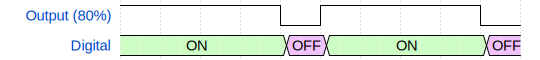
\includegraphics[scale=0.4]{generated_images/svg_generated/pwm.png}
    \caption{PWM Waveform}
    \label{fig:pwm_waveform}
\end{figure}

\noindent Note that PWM's application is not limited to LED's - in general, PWM can be thought of as a way to control the average voltage across a load, and is used in motor control, power supplies, and more.

\end{document}
